\documentclass[11pt,a4paper]{article}
\usepackage[T1]{fontenc}
\usepackage{lmodern}
\usepackage{a4wide}
\usepackage[dvips]{graphicx}
\usepackage{float}

\usepackage[
pdfauthor={ ACE Projekt Team },
pdftitle={ Evaluation Algorithms },
pdfcreator={pdftex},
]{hyperref}

\usepackage{sectsty}
\allsectionsfont{\sffamily}

\usepackage{fancyheadings} 
\pagestyle{fancy} 
\lhead{\textsf{\textbf{ACE} \\ \small{a collaborative editor}}}
\chead{}
\rhead{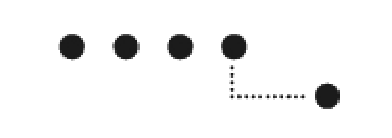
\includegraphics[height=0.875cm,width=3cm]{../../images/logo_BFH.eps}}
\lfoot{}
\cfoot{\textsf{\thepage}}
\rfoot{}
\setlength{\headrulewidth}{0.6pt}
\setlength{\footrulewidth}{0.6pt}
\setlength{\topmargin}{-50pt}
\addtolength{\headheight}{50pt}

\usepackage{colortbl}

\newcommand{\headercol}[2]{\multicolumn{1}{|>{\bfseries\columncolor[gray]{0.82}}p{#1}|}{\textsf{#2}}}
\newcommand{\ace}[0]{\emph{ACE }}



\begin{document}
\setlength{\parindent}{0pt}

\newtheorem{defn}{Definition}
\newtheorem{spec}{Specification}

\bibliographystyle{plain}

\begin{titlepage}
\thispagestyle{empty}
  \includegraphics[height=1.5in]{../../images/pix.eps}

  \begin{center}

    {\fontsize{40}{45} \textbf{\textsf{ACE}}} \\
    \textsf{a collaborative editor} \\
        
    \vspace{36pt}
        
    {\huge{\textbf{\textsf{Report Evaluation Network}}}} \\

    \vspace{36pt}

	\textsf{Berne University of Applied Sciences} \\
    \textsf{School of Engineering and Information Technology} \\
    
  \end{center}

  \vfill
  
  \begin{tabular}{ll}
   \hline

   \\

   \multicolumn{1}{>{\bfseries}p{1.5in}}{\textsf{Date:}} &
   \multicolumn{1}{>{}p{4.3in}}{\textsf{14.06.2005}}          \\
   
   \\
   
   \multicolumn{1}{>{\bfseries}p{1.5in}}{\textsf{Version:}}     &   
   \multicolumn{1}{>{}p{4.3in}}{\textsf{0.6}}                 \\

   \\
   
   \multicolumn{1}{>{\bfseries}p{1.5in}}{\textsf{Projectteam:}}                 &
   \multicolumn{1}{>{}p{4.3in}}{\textsf{Mark Bigler (biglm2@hta-bi.bfh.ch)}}  \\
   \multicolumn{1}{>{\bfseries}p{1.5in}}{}                                      &
   \multicolumn{1}{>{}p{4.3in}}{\textsf{Simon R�ss (rasss@hta-bi.bfh.ch)}}    \\
   \multicolumn{1}{>{\bfseries}p{1.5in}}{}                                      &
   \multicolumn{1}{>{}p{4.3in}}{\textsf{Lukas Zbinden (zbinl@hta-bi.bfh.ch)}} \\   
   
   \\
   
   \multicolumn{1}{>{\bfseries}p{1.5in}}{\textsf{Receivers:}}                       &
   \multicolumn{1}{>{}p{4.3in}}{\textsf{Jean-Paul Dubois (doj@hta-bi.bfh.ch)}}       \\
   \multicolumn{1}{>{\bfseries}p{1.5in}}{}                                          &
   \multicolumn{1}{>{}p{4.3in}}{\textsf{Claude Fuhrer (frc@hta-bi.bfh.ch)}}       \\

   \\
   
   \multicolumn{1}{>{\bfseries}p{1.5in}}{\textsf{Location:}}               &   
   \multicolumn{1}{>{}p{4.3in}}{\textsf{Subversion Repository}} \\

   \\  
   
   \hline
  \end{tabular}

\end{titlepage}

\newpage

\tableofcontents
\newpage
\listoftables
\listoffigures
\newpage


\section*{Versionskontrolle}

\begin{table}[!h]
 \begin{tabular}{|l|l|l|l|}
  \hline
  \headercol{0.6in}{Version}         & 
  \headercol{0.8in}{Datum}           &
  \headercol{1.2in}{Verantwortlich}  & 
  \headercol{2.8in}{Bemerkungen}     \\
  \hline
  0.1         & 15.03.2005  & zbinl           &  Erste Version \\
  0.2         & 16.03.2005  & Projektteam     &  �berarbeitung \\
  0.3         & 05.04.2005  & Projektteam     &  �berarbeitung vor Abgabe \\
  \hline
 \end{tabular}
 \caption{Versionskontrolle}
 \label{Versionskontrolle}
\end{table}

\begin{table}[!h]
 \begin{tabular}{|l|l|l|l|l|}
  \hline
  \headercol{0.9in}{}            & 
  \headercol{0.9in}{Stelle}      & 
  \headercol{0.8in}{Datum}       & 
  \headercol{0.6in}{Visum}       & 
  \headercol{2.0in}{Bemerkungen} \\
  \hline
  \textbf{Freigegeben}   & Projektteam &       &       &             \\
  \hline
  \textbf{Genehmigt}     &             &       &       &             \\
  \hline
 \end{tabular}
 \caption{Pr�fung/Genehmigung}
 \label{Pr�fung/Genehmigung}
\end{table}

\newpage


\section{Introduction}
Real-time cooperative editing systems allow multiple users to view and edit the same document at the same time from multiple sites connected by communication networks. Consistency maintenance is one of the most significant challenges in designing and implementing real-time cooperative editing systems. 


\subsection{Requirements}
The following requirements have been identified for such systems.

\paragraph{Real-time:} The response to local user actions must be quick, ideally as quick as a single-user editor, and the latency for reflecting remote user actions is low (determined by external communication latency only). 

\paragraph{Distributed:} Cooperating users may reside on different machines connected by communication networks with nondeterministic latency.

\paragraph{Unconstrained:} Multiple users are allowed to concurrently and independently edit any part of the document at any time, in order to facilitate free and natural information flow among multiple users.


\subsection{Preliminaries}
In this section, some basic concepts and terminologies are introduced. Following Lamport\cite{lamport78}, we define a causal (partial) ordering relation on operations in terms of their generation and execution sequences as follows.

\begin{defn}
Causal ordering relation $\rightarrow$
\end{defn}

Given two operations $O_{a}$ and $O_{b}$ generated at sites $i$ and $j$, then $O_{a}\rightarrow O_{b}$, iff:
\begin{enumerate}
 \item $i=j$ and the generation of $O_{a}$ happened before the generation of 
       $O_{b}$
 \item or $i \neq $j and the execution of $O_{a}$ at site $j$ happened before 
       the generation of $O_{b}$
 \item or there exists an operation $O_{x}$ such that $O_{a}\rightarrow O_{x}$
       and $O_{x}\rightarrow O_{b}$
\end{enumerate}

Note that the causal ordering relation is a \emph{partial ordering}.

\begin{defn}
Dependent and independent operations
\end{defn}

Given any two operations $O_{a}$ and $O_{b}$:
\begin{enumerate}
 \item $O_{b}$ is \emph{dependent} on $O_{a}$ iff $O_{a} \rightarrow O_{b}$
 \item $O_{a}$ and $O_{b}$ are \emph{independent} (or \emph{concurrent}), 
       expressed as $O_{a} \Arrowvert O_{b}$ iff neither 
       $O_{a}\rightarrow O_{b}$ nor $O_{b}\rightarrow O_{a}$
\end{enumerate}

Intuitively we can say that two operations are dependant if there exists a path from the generation of one message to the generation of another message. So for example in figure \ref{fig:example1} operation $O_{1}$ and $O_{3}$ are dependent, that is $O_{1}\rightarrow O_{3}$. Operation $O_{1}$ and $O_{2}$ are \emph{independent}. 


\subsection{A shared document model}
Consider $n$ sites, where each site has a copy of the shared document. The shared document model we take is a \emph{text document} modeled a by sequence of characters, indexed from 0 up to the number of characters in the document. It is assumed that the document state (the text) can only be modified by executing the following two primitive editing operations: (i) $Insert(p,c)$ which inserts the character $c$ at position $p$; (ii) $Delete(p)$ which deletes the character at position $p$.

It is important to note that the above text document model is only an abstract view of many document models based on a linear structure. For instance the character parameter may be regarded as a string of charcters, a line, a block of lines, an ordered XML node, etc.


\subsection{Three inconsistency problems}
\label{constraints}

To illustrate the challenges researchers are facing, consider a scenario in a cooperative editing system with three cooperating sites, as shown in figure \ref{fig:example1}. Suppose that an operation is executed on the local replica of the shared document immediately after its generation, then broadcast to remote sites and executed there in its \emph{original form} upon its arrival.
Three different inconsistency problems have been identified by {Sun et. al}\cite{sun98a}.

\begin{figure}
 \centering
 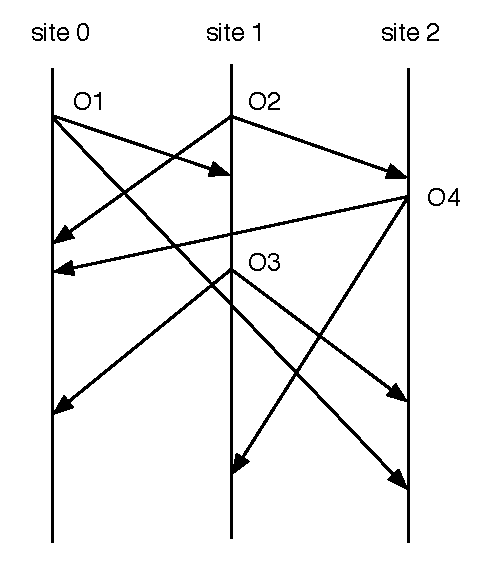
\includegraphics[width=2.5in,height=2.88in]{../../images/example1.eps}
 \caption{A scenarion of a real-time cooperative editing session}
 \label{fig:example1}
\end{figure}

\paragraph{Divergence:}
Operations may arrive and be executed at different sites in different orders, resulting in different final results. As shown in figure \ref{fig:example1}, the four operations in this scenario are executed in the following orders: $O_{1}$, $O_{2}$, $O_{4}$ and $O_{3}$ at site 0; $O_{2}$, $O_{1}$, $O_{3}$ and $O_{4}$ at site 1; and $O_{2}$, $O_{4}$, $O_{3}$ and $O_{1}$ at site 2. Unless operations are commutative, which is generally not the case, final editing results will diverge. The divergence problem can be solved by any serialization protocol, which ensures the final result is the same as if all operations were executed in the same total order at all sites.

\paragraph{Causality violation:}
Due to the nondeterministic communication latency, operations may arrive and be executed out of their natural cause-effect order. As shown in figure \ref{fig:example1}, operation $O_{3}$ is generated after the arrival of $O_{1}$ at site 1, the editing effect of $O_{1}$ on the shared document has been seen by the user 1 at the time $O_{3}$ is generated. Therefore, $O_{3}$ may be \emph{dependent} on $O_{1}$. However, since $O_{3}$ arrives and is executed before $O_{1}$ at site 2, confusion may occure to the system as well as to the user at site 2. For example, if $O_{1}$ is to insert a string into a shared document, and $O_{3}$ is to delete some characters in the string inserted by $O_{1}$, then the execution of $O_{3}$ before $O_{1}$ at site 2 will result in $O_{3}$ referring to a nonexistent context. 

\paragraph{Intention violation:}
Due to concurrent generation of operations, the \emph{actual effect} of an operation at the time of its execution may be different from the \emph{intended effect} of this operation at the time of its generation. As shown in figure \ref{fig:example1}, operation $O_{1}$ is generated at site 0 without any knowledge of $O_{2}$ generated at site 1, so $O_{1}$ is \emph{independent} of $O_{2}$, and vice versa. At site 0, $O_{2}$ is executed on a document state which has been changed by the preceding execution of $O_{1}$. Therefore, the subsequent execution of $O_{2}$ may refer to an incorrect position in the new document state, resulting in an editing effect which is different from the \emph{intention} of $O_{2}$. 

For example, assume the shared document initially contains the following sequence of characters: '"ABCDE'". Suppose $O_{1}=Insert['"12'",1]$, which intends to insert string '"12'" at position 1, i.e. between '"A'" and '"BCDE'"; and $O_{2}=Delete[2,2]$, which intends to delete the two characters starting from position 2, i.e. '"CD'". After the execution of these two operations, the \emph{intention-preserved} result (at all sites) should be: '"A12BE'". However, the actual result at site 0, obtained by executing $O_{1}$ followed by executing $O_{2}$, would be: '"A1CDE'", which apparently violates the intention of $O_{1}$ since the character '"2'", which was intented to be inserted, is missing in the final text, and violates the intention of $O_{2}$ since characters '"CD'", which were intended to be deleted, are still present in the final text.

Even if a serialization-based protocol was used to ensure that all sites execute $O_{1}$ and $O_{2}$ in the same order to get an identical result '"A1CDE'", but this identical result is still inconsistent with the intentions of both $O_{1}$ and $O_{2}$.

\paragraph{} 
The three inconsistency problems are independent in the sense that the occurence of one or two of them does not always result in the others. Particularly, intention violation is an incosistency problem of a different nature from the divergence problem. The essential difference between divergence and intention violation is that the former can always be resolved by a serialization protocol, but the latter cannot be fixed by any serialization protocol if operations were always executed in their originial forms.


\subsection{A consistency model}
A cooperative editing system is said to be consistent if it always maintains the following properties:
\paragraph{Convergence:} when the same set of operations have been executed at all sites, all copies of the shared document are identical.
\paragraph{Causality-preservation:} for any pair of operations $O_a$ and $O_b$, if $O_a \rightarrow O_b$, then $O_a$ is executed before $O_b$ at all sites.
\paragraph{Intention-preservation:} for any operation $O$, the effects of executing $O$ at all sites are the same as the intention of $O$, and the effect of executing $O$ does not change the effects of indepentent operations.

{\setlength{\parskip}{18pt}
In essence, the \emph{convergence} property ensures the consistency of the final results \emph{at the end} of a cooperative editing session; the \emph{causality-preservation} property ensures the consistency of the execution orders of dependent operations \emph{during} a cooperative editing session; and the \emph{intention-preservation} property ensures that executing an opertion at remote sites achieves the same effect as executing this operation at the local site at the time of its generation, and the execution effects of independent operations do not interfere with each other.
}

The consistency model imposes an execution order constraint on dependent operations only. The execution order of independent operations is left open as long as the convergence and intention-preservation properties are maintained. The consistency model effectively specifies, what assurance a cooperative editing system gives to its users and, what properties the underlying consistency maintenance mechanism must support.



\subsection{Operational Transformation}
{Ellis and Gibbs}~\cite{ellis} proposed a new kind of algorithm for consistency control, called \emph{Operational Transformation} (OT).  This kind of algorithm transforms operations to include/exclude the effects of other operations. Intuitively, transformation shifts the position parameter of an operation before execution to incorporate the effects of previously executed operations that it was not "aware" of (or that are concurrent) at the time of generation. Operational transformation helps to solve the problem of intention violation.

In general there are two different types of operational transformation, inclusion transformation (IT) and exclusion transformation (ET). All OT algorithms use inclusion transformation, whereas exclusion transformation is not needed by some algorithms.

A transformation function has to be defined for every combination of operations. So for a text editor with the primitive operations \emph{insert} and \emph{delete}, there would be a total of four transformation functions for IT and another four for ET. That is, given a transformation function T, T(\emph{insert, insert}), T(\emph{insert, delete}), T(\emph{delete, insert}) and T(\emph{delete, delete}) must be defined.

\subsubsection{Definitions}
\label{definitions}
Conceptually, an operation $O$ is associated with a \emph{context}, denoted as $CT_{O}$, which is the list of operations that need to be executed to bring the document from its initial state to the state on which $O$ is defined (\emph{definition context}). The significance of context is that the effect of an operation can be correctly interpreted only in its own context. If the current context (called \emph{execution context}) is different from the definition context of an operation, the operation has to be transformed so that it can be executed in the current context.

\begin{defn}
Context equivalent relation $\sqcup$
\end{defn}

Given two operations $O_{1}$ and $O_{2}$, associated with contexts $CT_{O_{1}}$ and $CT_{O_{2}}$ respectively, $O_{1}$ and $O_{2}$ are \emph{context-equivalent} iff $CT_{O_{1}}=CT_{O_{2}}$. Apparently, the context equivalent relation $\sqcup$ is transitive.

\begin{defn}
Context preceding relation $\mapsto$
\end{defn}
Given two operations $O_{1}$ and $O_{2}$ associated with contexts $CT_{O_{1}}$ and $CT_{O_{2}}$ respectively, $O_{1}$ is \emph{context preceding} $O_{2}$ iff $CT_{O_{2}}=CT_{O_{1}} + [O_{1}]$. Note that the contex preceding relation $\mapsto$ is not transitive by definition.

\subsubsection{Inclusion Transformation}
Inclusion Transformation (IT) transforms an operation $O_{1}$ against another operation $O_{2}$ in such a way that the impact of $O_{2}$ is effectively included. 
\begin{spec}
$IT(O_a,O_b):O'_a$
\end{spec}
\begin{enumerate}
 \item Precondition for input parameters: $O_a \sqcup O_b$
 \item Postcondition for output: $O_b \mapsto O'_a$ where $O'_a$'s execution effect in the context of $CT_{O'_a}$ is the same as $O_a$'s execution effect in the context of $CT_{O_a}$.
\end{enumerate}

Most important, it was recognized that the correctness of IT relies on the condition that both $O_{1}$ and $O_{2}$ are defined on the same document state so that their parameters are comparable and can be used to derive a proper adjustment to $O_{2}$, i.e. $O_{1} \sqcup O_{2}$.

\subsubsection{Exclusion Transformation}
Exlusion Transformation (ET) transforms an operation $O_{1}$ against another operation $O_{2}$ in such a way that the impact of $O_{2}$ is effectively excluded from $O_{1}$.
\begin{spec}
$ET(O_a,O_b):O'_a$
\end{spec}
\begin{enumerate}
 \item Precondition for input parameters: $O_b \mapsto O_a$
 \item Postcondition for output: $O_b \sqcup O'_a$ where $O'_a$'s execution effect in the context of $CT_{O'_a}$ is the same as $O_a$'s execution effect in the context of $CT_{O_a}$.
\end{enumerate}

Both transformation functions must meet the \emph{reversibility} requirement as defined next.

\subsubsection{Reversibility}
\begin{defn}
Reversibility Requirement
\end{defn}

Given two operations $O_{1}$ and $O_{2}$.

\begin{enumerate}
 \item if $O_{1} \sqcup O_{2}$ and $O'_{1} = IT(O_{1},O_{2})$, then it must
       be that $O_{1} = ET(O'_{1},O_{2})$
 \item if $O_{2} \mapsto O_{1}$ and $O'_{1} = ET(O_{1},O_{2})$, then it must
       be that $O_{1} = IT(O'_{1},O_{2})$
\end{enumerate}

Achieving reversibility is not a trivial task. This is because IT/ET functions may loose some information, so reversing the effect of a transformation may not be possible.


\subsection{Transformation Properties}
It was shown in \cite{ressel96} that transformation functions must satisfy two conditions, called $TP1$ and $TP2$. These transformation properties are sufficient and necessary for OT algorithms to guarantee convergence along arbitrary transformation paths.

\paragraph{Transformation Property 1:}
The transformation property 1 ensures that the effect of executing $O_{1}$ followed by the transformed request $O_{2}$ is the same as executing request $O_{2}$ followed by the transformed request $O_{1}$. 

\begin{defn}
Transformation Property 1:
$ O_{1} O'_{2} \equiv O_{2} O'_{1} $
\end{defn}

\paragraph{Transformation Property 2:}
Transformation property 1 is a necessary and sufficient condition to ensure that the groupware system with two users is correct. When there are more than two users, the situation is more complex. An operation can be transformed along different, albeit equivalent paths, not necessarily yielding the same result. In the simplest case, an operation can be transformed along the two paths of a simple transformation step. Operation $O_{1}$ may be transformed first with respect to $O_{2}$ and then to $O'_{3}$ yielding $IT(IT(O_{1},O_{2}),O'_{3})$, or it may be transformed first with respect to $O_{3}$ and then to $O'_{2}$ yielding $IT(IT(O_{1},O_{3}),O'_{2})$. Note that different sites might choose different paths for $O_{1}$ to be transformed. So we have to make sure that both paths lead to the same resulting operation:

\begin{defn}
Transformation Property 2: 
$IT(IT(O_{1},O_{2}),O'_{3})$=$IT(IT(O_{1},O_{3}),O'_{2})$
\end{defn}


\subsection{Groupware Architecture Analysis} We consider the architecture of a groupware application from two different point of views. On the one hand, the focus lies on the document replication and on the other, we consider the type of group communication between the participating sites.

\subsubsection{Document replication}

\paragraph{Centralized architecture} In a centralized architecture all data, i.e. the document, resides on a central machine. Client processes at each site are only responsible for passing requests to the central program and for displaying any output sent to them from the central program. The advantage of a centralized scheme is that synchronization is easy. Document state information is consistent since it is located in one place, and events are handled at clients in the same order because they are serialized by the server. Its main drawback is latency, as the message corresponding to any action must pass from the client to the server and back again before response to the action is shown.

\paragraph{Replicated architecture} In a replicated architecture the document is replicated at all participating sites. Client processes at each site (replicas) must coordinate explicitly both local and remote actions, synchronizing all copies of the document. Replicas need only exchange critical state information to keep their copy of the document current. While remote activities may still be delayed, local activities can be processed immediately. Processing bottlenecks are less likely, because each replica is responsible for drawing only the local view. The most significant cost of replication is increased complexity as issues of distributed systems like conflict management, concurrency control, etc. must be handled. 

The \emph{real-time} requirement has led most researchers to adopt a replicated architecture.


\subsubsection{Group Communication}
We consider two types of group communication architectures: unicast and multicast:

\paragraph{Unicast communication} Unicast communication is a two way communication where client processes at each site communicate bidirectionally with a centralized server. The server forwards information from one client to all other clients.

\paragraph{Multicast communication} Mulitcast communication is an $n$ way communication where client processes at each site communicate with all the participating sites directly. It has an enormous growth in terms of the number of communication paths. They grow at the rate of $n(n-1)/2$, where $n$ is the number of clients in the system. As compared to this, systems that use unicast communication have a linear growth. 


\section{History}
{Ellis and Gibbs}~\cite{ellis} were the first to propose an \emph{Operational Transformation} algorithm in 1989. The algorithm is called \emph{dOPT} and is implemented in the \emph{Grove} system. Soon however a flaw was discovered in the original \emph{dOPT} algorithm (by Cormack\cite{cormack95a}). The scenario where \emph{dOPT} failed is called the \emph{dOPT} puzzle. Ressel\cite{ressel96} proposed a new algorithm \emph{adOPTed} in 1996 that solved the original \emph{dOPT} puzzle. {Sun et. al}\cite{sun98a} proposed another algorithm called \emph{GOT} that similarly to \emph{adOPTed} solved the \emph{dOPT} puzzle. {Sun et. al}\cite{sun98b} developed some transformation functions for string-wise operations.

Later research groups\cite{imine03}\cite{imine04} proved the transformation functions of both Ressel\cite{ressel96} and Sun\cite{sun98a} to fail to hold TP2 in certain situations. They proposed new transformation functions they developed using a theorem prover. 

Proving the transformation property 1 (TP1) seems to be rather straightforward. However, proving that a given transformation function holds TP2 appears to be difficult. There are over 100 cases that have to be analyzed (according to {Imine et. al}\cite{imine04}). Imine et. al showed that many proposed transformation functions do not hold TP2. 

Recently, two different ways have been taken to deal with the TP2 problem. One kind of algorithms tries to avoid the need to comply with TP2 altogether (GOT~\cite{sun98a}, SOCT3/4~\cite{suleiman00}, TIBOT\cite{tibot} and NICE~\cite{sun02}). Other research groups~\cite{li04}~\cite{imine04} try to correct the problems in the original transformation functions of GOTO~\cite{sun98b}, adOPTed~\cite{ressel96} and SDT~\cite{sdt}. 


\section{Algorithms}
\label{algos}
In this section we give an overview of the \emph{Operational Transformation} algorithms we could gather. Two important properties on such algorithms are described first.

\paragraph{} The OT algorithm approach consists of two main components:

\begin{enumerate}
 \item The \emph{integration algorithm} which is responsible of receiving, broadcasting and executing operations. It is independent of the type of replica and application.
 \item The \emph{transformation function} is responsible for merging two concurrent operations. It is application dependent. For example, a text editor has different operations than a whiteboard application.
\end{enumerate}

The integration algorithm calls the transformation function when needed. The correctness of the OT approach relies on both the correct integration algorithm as well as on the correct transformation function.

\subsection{dOPT}
\label{algo:dopt}

\emph{dOPT} (Distributed Operational Transformation) is the first operational transformation algorithm developed by {Ellis and Gibbs}\cite{ellis} in 1989. It was soon discovered that in some situations the document replicas did not converge. This situation is known as the \emph{dOPT} puzzle.

The algorithm fails in cases where there is more than one concurrent operation from a user. Gormack\cite{cormack95a} detected this case and proposed a new algorithm (see \ref{algo:ccu}) that is only suitable for two sites connected by a point-to-point communication channel. He stated that there does not appear to be a simple and efficient correction to \emph{dOPT} that maintains its suitability for broad-cast operations.

However Gormack showed in \cite{cormack95b} that using several point-to-point communication channels forming a tree it is possible to derive a consistent solution for an arbitrary number of sites.

\subsubsection{Properties}
\begin{itemize}
 \item algorithm is incorrect
 \item uses state vectors to maintain causal ordering
 \item uses linear history buffer (called request log)
 \item architecture: fully replicated
\end{itemize}

\subsection{CCU}
\label{algo:ccu}

CCU (a Calculus for Concurrent Update) derives from the \emph{dOPT} (see \ref{algo:dopt}) algorithm. It was developped by Gordon V.Cormack in 1995 that discovered earlier \cite{cormack95a} that \emph{dOPT} is incorrect. 

The algorithm specifies a concurrent model based on a sequential model augmented with definitions of all possible pairs of elementary operations (updates). The concurrent model is implemented by a set of objects: one for each source of events.

Although there is a description of the algorithm in \cite{cormack95b}, many implementation details are left out. The only information is given is that the simplest n-site algorithm is a star built from multiple versions of the 2-site implementation.

Interestingly no references to this algorithm are found in the research material from other researchers. 

\subsubsection{Properties}
\begin{itemize}
 \item correctness never confirmed by other reaserchers
 \item uses state vectors to maintain causal ordering
 \item architecture: semi-replicated (central server)
\end{itemize}

\subsection{Jupiter}
\label{algo:jupiter}

\emph{Jupiter} is a multi-user, multimedia virtual world intended to support long-term remote collaboration. In particular, it supports shared documents, shared tools, and, optionally, live audio/video communication. The low-level communication facilities are described in \cite{jupiter95}.

The state of the \emph{Jupiter}, including application code written by users, is stored and (for code) executed in a central server shared by all users. This architecture was chosen to support multiple client platforms and high-latency networks. Clients and servers communicate in terms of high-level widgets and user events.

\emph{Jupiter}'s algorithm is derived from \emph{dOPT}. The centralized architecture and thus the reduction of point-to-point connections allows them to simplify the \emph{dOPT} algorithm. Several point-to-point connections are used to build a tree-structured $n$-site algorithm.

\emph{Jupiter} solves the \emph{dOPT} puzzle. It uses a two dimensional state space instead of a linear history buffer (request log) to save operations. It transforms saved messages when there are incoming messages. Unfortunately, simply transforming saved messages does not work for the $n$-way case, since the next message can come from a third site that is in an inconvenient message state.

The algorithm labels each message with the state the sender was in just before the message was generated. The recipient uses these labels to detect conflicts. Two concurrent messages have to be transformed, but they can only be transformed  when they were generated from the same state of the document. Otherwise, special handling is required.


\subsubsection{Properties}
\begin{itemize}
 \item seems to be correct
 \item uses state vectors to decide causality relations
 \item architecture: semi-replicated (central server)
 \item uses multiple 2-way synchronization protocols to create a n-way protocol
\end{itemize}

\subsection{NetEdit Consistency Algorithm}
\label{algo:netedit}

\emph{NetEdit} is a collaborative text editor (\cite{netedit}) that uses a replicated architecture with processing and data distributed across all clients. It uses an $n$-way synchronization protocol derived from the algorithm of the \emph{Jupiter} (see \ref{algo:jupiter}) collaboration system. The algorithm is called \emph{NetEdit Consistency Algorithm}.

The 2-way synchronization protocol developed for \emph{Jupiter} was the starting point. That algorithm was extended to a multi-way protocol using multiple 2-way connections. All the clients maintain a state-space graph. This state-space is used to maintain information where the other is in the editing process. Both client and server pass through this state space as they process messages.

The algorithm labels each message with the state the sender was in just before the message was generated. The recipient uses these labels to detect conflict. Two concurrent messages have to be transformed, but they can only be transformed  when they were generated from the same state of the document. Otherwise, special handling is required.

It is not clear how this algorithm differs from \emph{Jupiter} as \emph{Jupiter} was obviously extended to an n-way synchronization protocol using a similar (the same?) approach.


\subsubsection{Properties}
\begin{itemize}
 \item seems to be correct
 \item uses state vectors to decide if operations are concurrent
 \item architecture: semi-replicated (central server)
 \item uses multiple 2-way synchronization protocols to create a n-way protocol
\end{itemize}


\subsection{adOPTed}
\label{algo:adopted}

\subsection{GOT}
\label{algo:got}

\subsection{GOTO}
\label{algo:goto}

\subsection{SOCT2}
\label{algo:soct2}

\subsection{SOCT3}
\label{algo:soct3}

Verifying that a given set of transformation functions satiesfies transformation property 2 (TP2) is not trivial. There are over a hundred cases to be checked depending on the various parameters. So the inventors of \emph{SOCT3} and \emph{SOCT4} (see \ref{algo:soct4}) decided to go a different way in order that  TP2 must not hold (\cite{suleiman00}).

They propose the implementation of a global serialization order such that the operations can be delivered in this order. The global serialization order is achieved by the use of a sequencer (see \ref{sequencer}). A sequencer is an object which delivers continously growing positive integer values, called timestamps. A timestamp is obtained through a call to a function \emph{Ticket}.

A local operation $O$ is executed immediately to respect the real-time constraint. Next, the call to the function \emph{Ticket} returns a timestamp $N_{O}$ which is assigned to the operation. The quadruplet $<O,S_{O},V_{O},N_{O}>$ is then broadcast where $V_{O}$ is the state vector associated with $O$ and $N_{O}$.

The reception procedure ensures a sequential delivery of all operations with respect to the ascending order of the timestamps. Upon receiving an operation it delays its delivery until all operations with lower timestamps have been received and delivered. The state vector is of no use for the reception procedure, but it enables to determine which operations are concurrent to $O$ during the integration step.

\emph{SOCT3} uses both inclusion transformation IT (called forward transposition) and exclusion transformation ET (called backward transposition) in the integration step. For details, see \cite{suleiman00}.


\subsubsection{Properties}
\begin{itemize}
 \item uses state vectors to determine causal relations
 \item uses linear history buffer (called history)
 \item architecture: fully replicated
 \item uses a unique global ordering to abandon TP2 (by using a sequencer)
 \item no known user undo algorithm
\end{itemize}

\subsection{SOCT4}
\label{algo:soct4}

In \emph{SOCT4} (\cite{suleiman00}) as in \emph{SOCT3}, the operations are ordered globally using a timestamp given by a sequencer. They are then delivered on each site in this order thanks to the sequential reception. The originality of \emph{SOCT4} comes from the fact that inclusion transformation (called forward transposition) that takes into account concurrent operations are now made by the generator sites of the operations. According to \cite{suleiman00} this results in three major advantages:

\begin{enumerate}
 \item the receiver site does not have to separate history anymore; 
       thus backward transposition becomes unecessary
 \item the received operation can be stored as it is in the history
       without further transformation
 \item state vectors are no longer needed
\end{enumerate}

To achieve this, the broadcast of an operation must be deferred until it has been assigned a timestamp and all the operations which precede it according to the timestamp order have been received and executed. As usual, local operations are executed immediately without delay.


\subsubsection{Properties}
\begin{itemize}
 \item does not need any state vectors
 \item architecture: fully replicated
 \item uses a unique global ordering to abandon TP2 (by using a sequencer)
 \item no exclusion transformation needed
 \item no known user undo algorithm
\end{itemize}


\subsubsection{Sequencer}
\label{sequencer}
As noted before, both \emph{SOCT3} and \emph{SOCT4} use sequencer to globally serialize operations. In \emph{SOCT4} operations are broadcast sequentially. This makes collaboration difficult when the propagation delay of an operation on the network is high. This characteristic makes \emph{SOCT4} particularly adapted to fast networks.

More information about sequencers can be found in \cite{reed79}. Various methods for implementing sequencers are described in \cite{lelann78} (circulating sequencers) and \cite{banino79} (replicated sequencers).

\subsection{TIBOT}
\label{algo:tibot}


\subsection{NICE}
\label{algo:nice}

Haifeng Shen and Chengzhen Sun devised a new operational transformation control algorithm in combination with a notification component in 2002 \cite{sun02}. In this paper they describe a flexible notification framework that can be used to implement a wide range of notification strategies used in collaborative systems.

In the proposed framework, the notification policy that determines when and what to notify is separated from the notification mechanism that determines how to notify. The parameters \emph{frequency} and \emph{granularity} are provided to define various notification policies. 

The frequency parameter determines the \emph{when} aspect of notification, that is, when a notification is propagated/accepted. The granularity parameter determines the \emph{what} aspect of notification, that is, which updates are going to be propagated/accepted. Further there can be a separate policy for input and output direction.

The notification mechanism determines the \emph{how} aspect. Both outgoing and incoming messages are put in distinct buffers (input buffer IB and output buffer OB). An outgoing notification executor (ONE) and an incoming notification executor (INE) are needed to carry out various outgoing and incoming notification policies respectively.

A very important component in the notification mechanism is the notification propagation protocol (NPP), which is needed for propagating updates from the OB at the notifying site to the IB at the notified site.

The notifications are contextually serialized. This is achieved by use of a central notification server, which acts as a centralized serialization point and message relaying agent (all messages pass through this central server). 


\subsubsection{Notification Propagation Protocol}
Before propagating a notification, the notifying site sends a \emph{Token-Request} message to the \emph{Notifier}, waiting for the \emph{Token-Grant} message from the \emph{Notifier}. After being granted the token, the site propagates the notification piggybacked with the \emph{Token-Release} message to the \emph{Notifier}. When the \emph{Notifier} receives the notification and the \emph{Token-Release} message, it forwards the notification to all interested sites. By using the notifier as a message relaying agent, causal relationships among notifications are automatically guaranteed.

This sequential propagation simplifies concurrency control. However it is also inefficient for supporting notification policies for meeting real-time collaboration needs. For propagating one notification that may contain only one operation, three extra messages have to be sent.


\subsubsection{Concurrent Propagation}
So the proposed solution consists of a protocol that allows a site to propagate its notification without first requesting a token, thus effectively eliminating the \emph{Token-Request} message. This operation propagation protocol is called \emph{SCOP} (symmetric contextually-serialized operation propagation). 


\subsubsection{Properties}
The transformation control algorithm is called \emph{SLOT} (symmetric linear operation transformation). Together with the \emph{SCOP} protocol it has the following properties.

\begin{itemize}
 \item architecture: semi-replicated (uses central notification server)
 \item no state vectors needed
 \item no exclusion transformation (ET)
 \item free of transformation property 2 (TP2)
\end{itemize}

The reason why \emph{SLOT} is free of TP2 is that under no circumstance an operation could be transformed against the same pair of operations in different orders. The operation are always ordered uniquely.


\subsection{SDT}
\label{algo:sdt}

The algorithm \emph{SDT} was presented in 2004 by Du Li and Rui Li \cite{sdt}. They detected defects in existing inclusion transformation and exclusion transformation functions. The proposed solution (\emph{SDT}) tries to fix these.

\subsubsection{Defects of traditional transformation functions}
The problem is related to inclusion transformation between two insert operations and one delete operation with close position parameters. In some of these cases, the result of inclusion transformation is not deterministic. 

\paragraph{Example: } Given the initial document state ''abc''. The three editing sites 1, 2 and 3 generate $O_{1} = insert(''1'',2)$, $O_{2} = insert(''2'',1)$ and $O_{3} = delete(''b'',1)$ respectively. The three operations are independent. Now consider what happens at site 3. After the deletion of character ''b'' at position 1 the document state becomes ''ac''. The next message arriving is then $O_{2}$ which inserts ''2'' at position 1. The resulting document state is ''a2c''. The next operation $O_{1}$ arrives at site 3 and is transformed against $O_{3}$ and then $O_{2}$. The result of the second transformation is non-deterministic. It could be $insert(''1'',1)$ or $insert(''1'',2)$. However, the original intention of $O_{1}$ is to insert ''1'' after ''b'' and the intention of $O_{2}$ is to insert ''2'' before ''b''. Then ''1'' should appear after ''2'' in the resulting document state (''a21c''). So depending on the chosen priority scheme, the result could be violating the intention of the original operations. Another even more severe problem results from the fact, that the document state of site 3 could diverge from site 1 and 2. A similar problem arises with traditional exclusion transformation functions.

The conventional transformation functions use the site id as priority scheme if two inserts happen at the same position. This was identified as the source of the problems as described above by Du Li and Rui Li. This new algorithm tries to delay the use of site ids.


\subsubsection{Proposed Solution}
The algorithm works conceptually as follows. For each operation the original intention is recovered by computing its $\beta$ value against a well-known document state (the latest synchronization point). Then in performing inclusion transformation, the $\beta$ values are compared. An algorithm to compute $\beta$ is given in the paper. The approach is based on a new concept called state difference, hence the name \emph{SDT} (state difference transformation).

The user intention is always achieved through performing operations that generate certain effects on a given document state. The effect of an operation $O$ on its definition context is trivially itself, either to insert or delete a character. However, the effect of operation $O$ on $S_{i}$ is not as obvious if $S_{i}$ precedes the definition context. To characterize the effect of an operation on a prior document state more accurately, two notations $\beta$ and $\delta$ are introduced.

Read \cite{sdt} for a general overview and \cite{li03} for the implementation details. The former document does not specify important implementation details (e.g. it is not explained how to obtain the \emph{latest synchronization point}). We did not read \cite{li03} because \emph{SDT} was proved incorrect \cite{imine04} and we did not find the document on the Internet.

\subsubsection{Properties}
\begin{itemize}
 \item transformation functions must hold TP2
 \item no undo mechanism
 \item proposed IT/ET functions proved wrong by Imine et. al \cite{imine04}, 
       i.e. they do not hold TP2 in all cases
 \item architecture: replicated, multicast
\end{itemize}




\section{Li04}
\label{algo:li04}


\newpage

\section{Comparison of Algorithms}

\subsection{Overview}

The following tables compare different aspects of the examined algorithms. The first table explains what is meant by the aspects.

\newcommand{\acol}[1]{\multicolumn{1}{|p{1.6in}|}{\small{#1}}}
\newcommand{\dcol}[1]{\multicolumn{1}{|p{3.9in}|}{\small{#1}}}

 \begin{table}[!ht]
  \begin{tabular}{|l|c|}
   \hline
    \headercol{1.6in}{Aspect} & 
    \headercol{3.9in}{Description}  \\
   \hline
    \acol{Year} & 
    \dcol{The year the research paper was published.} \\
   \hline 
    \acol{Correct?} & 
    \dcol{No if another research paper has proved the algorithm (or its OT functions) wrong, otherwise Yes} \\
   \hline 
    \acol{Architecture} & 
    \dcol{Which architecture is the algorithm designed for?} \\
   \hline 
    \acol{Available Information} & 
    \dcol{Is there enough information for an implementation?} \\
   \hline 
    \acol{Intention Preservation} & 
    \dcol{How is the user's intention for an operation be preserved? (see \ref{constraints})} \\
   \hline 
    \acol{Causality Preservation} & 
    \dcol{How is causal ordering relation on operations preserved? (see \ref{constraints})} \\
   \hline 
    \acol{Copies Convergence} & 
    \dcol{How is copy convergence on all replicated objects achieved? (see \ref{constraints})} \\
   \hline 
    \acol{Broadcast} & 
    \dcol{When is the broadcast i.e. the emission of a generated operation carried out?} \\
   \hline 
    \acol{Delivery} & 
    \dcol{In what order are the operations at each site executed?} \\
   \hline 
    \acol{Undo} & 
    \dcol{Is a user undo functionality for the algorithm available?} \\
   \hline
  \end{tabular}
  \caption{Aspect Explanation}
 \end{table}

\newcommand{\ccol}[1]{\multicolumn{1}{|p{0.8in}|}{\tiny{#1}}}

\begin{table}[H]
 \begin{tabular}{|l|c|c|c|c|c|}
  \hline
   \headercol{0.8in}{} &
   \headercol{0.8in}{dOPT} &
   \headercol{0.8in}{Jupiter} &
   \headercol{0.8in}{adOPTed} &
   \headercol{0.8in}{GOT} &
   \headercol{0.8in}{GOTO} \\
  \hline
  \hline
   \ccol{Year} &
   \ccol{1989} &
   \ccol{1995} &
   \ccol{1996} &
   \ccol{1998} &
   \ccol{1998} \\
  \hline
   \ccol{Correct?} &
   \ccol{no} &
   \ccol{control algorithm} &
   \ccol{control algorithm} &
   \ccol{yes} &
   \ccol{control algorithm} \\
  \hline
   \ccol{Architecture} &
   \ccol{replicated, multicast} &
   \ccol{replicated, unicast} &
   \ccol{replicated, multicast} & 
   \ccol{replicated, multicast} &
   \ccol{replicated, multicast} \\
  \hline
   \ccol{Available Information} &
   \ccol{enough} &
   \ccol{enough} &
   \ccol{enough} & 
   \ccol{enough} &
   \ccol{enough} \\
  \hline
  \hline
   \ccol{Intention Preservation} &
   \ccol{dOP Transformation} &
   \ccol{Transformation and two-dimensional graph} &
   \ccol{L-Transformation and multidimensional graph} &
   \ccol{IT and ET} &
   \ccol{IT and ET} \\
  \hline 
   \ccol{Causality Preservation} &
   \ccol{state vectors} &
   \ccol{state vectors} &
   \ccol{state vectors} &
   \ccol{state vectors} &
   \ccol{state vectors} \\
  \hline
   \ccol{Copies Convergence} &
   \ccol{TP1 (but no convergence achieved)} &
   \ccol{TP1} &
   \ccol{TP1 and TP2} &
   \ccol{non-continuous global order and undo/redo} &
   \ccol{TP1 and TP2} \\
  \hline
  \hline
    \ccol{Broadcast} &
    \ccol{immediate} &
    \ccol{immediate} &
    \ccol{immediate} &
    \ccol{immediate} &
    \ccol{immediate} \\
  \hline
   \ccol{Delivery} &
   \ccol{causal order} &
   \ccol{causal order} &
   \ccol{causal order} &
   \ccol{causal order} &
   \ccol{causal order} \\
  \hline
  \hline
   \ccol{Undo} &
   \ccol{no} &
   \ccol{no (but could be derived from adOPTed)} &
   \ccol{yes} &
   \ccol{no} &
   \ccol{yes} \\
  \hline
 \end{tabular}
 \caption{Comparison Matrix 1}
\end{table}

\begin{table}[H]
 \begin{tabular}{|l|c|c|c|c|c|}
  \hline
   \headercol{0.8in}{} &
   \headercol{0.8in}{SOCT2} &
   \headercol{0.8in}{SOCT3} &
   \headercol{0.8in}{SOCT4} &
   \headercol{0.8in}{SDT} &
   \headercol{0.8in}{TIBOT} \\
  \hline
  \hline
   \ccol{Year} &
   \ccol{1997} &
   \ccol{2000} &
   \ccol{2000} &
   \ccol{2004} &
   \ccol{2004} \\
  \hline
   \ccol{Correct?} &
   \ccol{no (transformation functions)} &
   \ccol{yes} &
   \ccol{yes} &
   \ccol{no (transformation functions)} &
   \ccol{yes} \\
  \hline
   \ccol{Architecture} &
   \ccol{replicated, multicast} &
   \ccol{replicated, multicast} &
   \ccol{replicated, multicast} & 
   \ccol{replicated, multicast} &
   \ccol{replicated, multicast} \\
  \hline
   \ccol{Available Information} &
   \ccol{enough} &
   \ccol{implementation of sequencers} &
   \ccol{implementation of sequencers} & 
   \ccol{not enough for implementation} &
   \ccol{not enough} \\
  \hline
  \hline
   \ccol{Intention Preservation} &
   \ccol{IT and ET} &
   \ccol{IT and ET} &
   \ccol{only IT} &
   \ccol{IT and ET} &
   \ccol{IT} \\
  \hline 
   \ccol{Causality Preservation} &
   \ccol{state vectors} &
   \ccol{timestamps} &
   \ccol{timestamps} &
   \ccol{state vectors} &
   \ccol{time intervals} \\
  \hline
   \ccol{Copies Convergence} &
   \ccol{TP1 and TP2} &
   \ccol{TP1 and continous global order} &
   \ccol{TP1 and continous global order} &
   \ccol{TP1 and TP2} &
   \ccol{TP1, propagation and synchronization rules} \\
  \hline
  \hline
    \ccol{Broadcast} &
    \ccol{immediate} &
    \ccol{immediate (as soon as timestamp is assigned)} &
    \ccol{deferred, in timestamp order} &
    \ccol{immediate} &
    \ccol{deferred, after time interval} \\
  \hline
   \ccol{Delivery} &
   \ccol{causal order} &
   \ccol{continous global order} &
   \ccol{continous global order} &
   \ccol{causal order} &
   \ccol{?\footnotemark} \\
  \hline
  \hline
   \ccol{Undo} &
   \ccol{no} &
   \ccol{no} &
   \ccol{no} &
   \ccol{no} &
   \ccol{no} \\
  \hline
 \end{tabular}
 \caption{Comparison Matrix 2}
\end{table}
\footnotetext{Due to lack of information we are not capable of determining the answer definitely.}

\begin{table}[H]
 \begin{tabular}{|l|c|c|c|c|c|}
  \hline
   \headercol{0.8in}{} &
   \headercol{0.8in}{NICE} &
   \headercol{0.8in}{LI04} &
   \headercol{0.8in}{CCU} &
   \headercol{0.8in}{} &
   \headercol{0.8in}{} \\
  \hline
  \hline
   \ccol{Year} &
   \ccol{2002} &
   \ccol{2004} &
   \ccol{1995} &
   \ccol{} &
   \ccol{} \\
  \hline
   \ccol{Correct?} &
   \ccol{yes} &
   \ccol{yes} &
   \ccol{probably yes} &
   \ccol{} &
   \ccol{} \\
  \hline
   \ccol{Architecture} &
   \ccol{replicated, unicast} &
   \ccol{replicated, multicast} &
   \ccol{replicated, unicast} & 
   \ccol{} &
   \ccol{} \\
  \hline
   \ccol{Available Information} &
   \ccol{enough} &
   \ccol{not enough \footnotemark} &
   \ccol{not enough} & 
   \ccol{} &
   \ccol{} \\
  \hline
  \hline
   \ccol{Intention Preservation} &
   \ccol{IT} &
   \ccol{IT and ET} &
   \ccol{?} &
   \ccol{} &
   \ccol{} \\
  \hline 
   \ccol{Causality Preservation} &
   \ccol{central notification server} &
   \ccol{state vectors} &
   \ccol{?} &
   \ccol{} &
   \ccol{} \\
  \hline
   \ccol{Copies Convergence} &
   \ccol{TP1 and unique global order} &
   \ccol{TP1 and TP2} &
   \ccol{TP1 and TP2} &
   \ccol{} &
   \ccol{} \\
  \hline
  \hline
    \ccol{Broadcast} &
    \ccol{immediate} &
    \ccol{immediate} &
    \ccol{immediate} &
    \ccol{} &
    \ccol{} \\
  \hline
   \ccol{Delivery} &
   \ccol{causal order} &
   \ccol{causal order} &
   \ccol{causal order} &
   \ccol{} &
   \ccol{} \\
  \hline
  \hline
   \ccol{Undo} &
   \ccol{no} &
   \ccol{no} &
   \ccol{no} &
   \ccol{} &
   \ccol{} \\
  \hline
 \end{tabular}
 \caption{Comparison Matrix 3}
\end{table}
\footnotetext{The paper \cite{li04a} with the necessary implementation details should be released around May 2005.}

\subsection{Selection Criteria}

From the set of available algorithms we want to make a pre-selection. This pre-selection is based on the criteria set forth in this section.

\paragraph{Correctness:} This is obviously the most important criteria. If an algorithm is not correct, it is not worth being implemented.

\paragraph{Availability of information:} Some papers do not provide enough information for an implementation.

\paragraph{Availability of user undo:} Users of collaborative applications expect the same commands as in a single user application. Without user level undo, the user experience will not be satisfactory.

\paragraph{Algorithmic complexity:} Some algorithms are strikingly simple, others are very complex (too complex). Simplicity is a selection criteria.


\subsection{Selection of Algorithms}

\subsubsection{Correctness}
Based on the first selection criteria (correctness) \emph{dOPT} algorithm is deemed unsuitable. Further the transformation functions used by some algorithms have been proved incorrect \cite{imine04}. These include \emph{adOPTed}, \emph{GOTO}, \emph{SOCT2} and \emph{SDT}. Note that the transformation functions can be replaced as they are independent of the control algorithm. By using the proposed IT function of \cite{imine04} these control algorithms would be correct again (at least the control algorithm of \emph{adOPTed} and \emph{GOTO} have been proved correct). As \emph{GOTO}, \emph{SOCT2} and \emph{SDT} also use ET functions and \cite{imine04} only proposed and proved IT, we cannot assume them to be correct for an implementation yet. There have to be ET functions developed and proved analogous to the IT functions in \cite{imine04} first.

The following algorithms meet the correctness criteria:
\begin{itemize}
 \item \emph{Jupiter}
 \item \emph{adOPTed}
 \item \emph{GOT}
 \item \emph{SOCT 3/4}
 \item \emph{TIBOT}
 \item \emph{NICE}
 \item \emph{LI04}
 \item \emph{CCU}
\end{itemize}

It is important to note that \emph{CCU}, \emph{TIBOT} and \emph{LI04} have not been approved or successfully implemented by a third party as far as we know.


\subsubsection{Availability of Information}
For the algorithms in the next list we do not have enough information available for an implementation.

\begin{itemize}
 \item \emph{CCU} (see \ref{algo:ccu})
 \item \emph{SDT} (see \ref{algo:sdt})
 \item \emph{TIBOT} (see \ref{algo:tibot})
\end{itemize}

For the implementation of \emph{SOCT3} and \emph{SOCT4} some more papers are needed concerning the implementation of sequencers. Though referenced, these could not be found on the Internet. 

For \emph{Li04} we do not have enough information yet. But there will be a paper with implementation details published around May 2005 according to Mr. Du Li.


\subsubsection{Complexity}
\emph{SOCT2} is considered to be very complex \cite{imine03b} \cite{sdt} due to management of the sets $s_i$ and $b_i$ associated with each $Insert$ operation. \emph{SOCT3} and \emph{SOCT4} use a sequencer that simplifies the implementation of the algorithm but requires this additional component which complicates the implementation. The theoretical aspects of \emph{GOT} as well as \emph{GOTO} are relatively complex, but the implementation itself should be straightforward. \emph{NICE} uses a central notification server that simplifies the algorithm significantly. \emph{Jupiter} is a very simple algorithm, because it restricts itself to point-to-point communication. \emph{adOPTed} is more complicated than \emph{Jupiter} because it adds $n$-way communication. However, we consider the implementation as relatively straightforward.  

The following algorithms are considered to be too complex to be accounted for an implementation.
\begin{itemize}
 \item \emph{SOCT2}
\end{itemize}


\subsubsection{User Undo}
The following algorithms have a user level undo defined. This does not imply that it would be impossible to devise an undo mechanism for other algorithms. Note however that adding an undo mechanism to an existing algorithm is a non-trivial task.

\begin{itemize}
 \item \emph{Jupiter} (see \ref{algo:jupiter}) 
 \item \emph{adOPTed} (see \ref{algo:adopted})
 \item \emph{GOTO} (see \ref{algo:goto})
\end{itemize}


\subsubsection{Selected Algorithms}
Based on the above observations but excluding the user undo requirement, the following algorithms remain as implementation choice:

\begin{itemize}
 \item \emph{Jupiter} (see \ref{algo:jupiter})
 \item \emph{adOPTed} (see \ref{algo:adopted})
 \item \emph{GOT} (see \ref{algo:got})
 \item \emph{NICE} (see \ref{algo:nice})
\end{itemize}

If we take the user undo functionality into account, the selection shrinks to three algorithms:
\begin{itemize}
 \item \emph{Jupiter} (see \ref{algo:jupiter}) 
 \item \emph{adOPTed} (see \ref{algo:adopted})
\end{itemize}

All the above algorithms fulfill the selection criteria sufficently well.


\newpage

\section{Transformation Functions}
In section \ref{algos}, we described several control algorithms along with their proposed transformation functions. Additionally, there exist research papers which focus only on transformation functions which are considered to be used with existing control algorithms. In this section we summarize the research papers we have found on that topic.


\subsection{IT function based on position words}
\label{otf:imor}

A new approach to achieving convergence is presented by A. Imine et al. in \cite{imine04}. They have formally proved the proposed solution to be correct. Firstly, the key concept of position words is introduced. Secondly, the novel IT function is explained.

\subsubsection{Position Words}
\paragraph{Definition p-word} Let $\Sigma = N$ be an alphabet over natural numbers. The set $\cal P \subset N^*$ of words, called p-words, is defined as follows: (i) $\epsilon \in \cal P$; (ii) if n $\in$ N then n $\in \cal P$; (iii) if $\omega$ is a nonemtpy p-word and n $\in$ N then n$\omega \in \cal P$ iff either n = Current($\omega$) or Current($\omega$) $\pm$ 1. Current($\omega$) is denoted the first symbol of $\omega$. Thus, Current(1232) = 1.

The position word (p-word) is a vector of numbers which is denoted by $\omega$ and defined only on insertion operations. This vector keeps track of the insertion positions of an operation. E.g. p-words are $\omega_{1}$ = 00, $\omega_{2}$ = 3454, but $\omega_{3}$ = 3476 is not. 

\subsubsection{IT function}
The insert operation is extended with a new parameter p-word giving the positions occupied before every transformation step. Thus an insert operation becomes: $Ins(p,c,w)$ where $p$ is the insertion position, $c$ the character to be added and $w$ a p-word.

The OT function is redefined using the p-word concept. A function PW is defined that enables to construct p-words from editing operations. Hence, given an insert operation op, PW(op) gives a p-word which restores all positions occupied by the insert operation op since it was generated. 

When the OT function for two insertion operations is called, the PW values of $Ins(p_1,c_1,w_1)$ and $Ins(p_2,c_2,w_2)$ are first compared. If their p-words are equal, then their character codes are compared. When the two operations have the same character to be inserted in the same position then the OT function gives the null operation nop, i.e. one insert operation must be executed and the other one must be ignored \cite{suleiman98}.

\subsubsection{Properties}
\begin{itemize}
 \item IT function extended with concept of p-words
 \item p-word: a vector of positions an insertion operation has undergone since its generation
 \item first (inclusion) transformation function which was thoroughly formally proved ever
 \item has been successfully implemented with algorithm adOPTed in \cite{cicolini} and SOCT4 in \cite{mosi}
\end{itemize}

\subsection{IT and ET for stringwise operations}
\label{otf:sun}

\subsubsection{Properties}
\begin{itemize}
 \item 
\end{itemize}


\newpage

\appendix
\section{ Appendix }
code fragments

\newpage
\bibliography{ace}

\end{document}

